\documentclass[12pt]{article}
\usepackage{amsmath}
\usepackage{amsthm}
\usepackage{amsfonts}
\usepackage{amssymb}
\usepackage{enumerate}
\usepackage{graphicx}
\usepackage{mdframed}
\usepackage{multicol}
\usepackage{verbatim}
\usepackage{tikz}
\usepackage{pdfpages}
\usepackage[margin = .8in]{geometry}
\geometry{letterpaper}
\linespread{1.2}

\newcommand{\RR}{\mathbb{R}}
\newcommand{\NN}{\mathbb{N}}
\newcommand{\ZZ}{\mathbb{Z}} 
\newcommand{\QQ}{\mathbb{Q}}

\newcommand\set[1]{\left\lbrace #1 \right\rbrace}
\newcommand\abs[1]{\left| #1 \right|}
\newcommand\parens[1]{\left( #1 \right)}
\newcommand\brac[1]{\left[ #1 \right]}
\newcommand\sol[1]{\begin{mdframed}
\emph{Solution.} #1
\end{mdframed}}
\newcommand\solproof[1]{\begin{mdframed}
\begin{proof} #1
\end{proof}
\end{mdframed}}

\begin{document}
\noindent Theodore Nguyen \hfill Due July 10\textsuperscript{th} 11:55 pm

\begin{center}
  {\large Introduction to Machine Learning \\ Assignment Paper \#1}
\end{center}

\section*{Part I: Reflection on your learning (20pt)}
\begin{enumerate}[(1)]
    \item What have you learned in the class so far?
    \begin{mdframed}
        I've learned about the differences between supervised and unsupervised learning. I've also learned what \texttt{accuracy}, \texttt{precision}, and \texttt{recall} mean and how to calculate them. I've learned the general concept behind $k$-Nearest Neighbors and how to use Python to execute the algorithm.
    \end{mdframed}
    \item Which area (knowledge, skillset, attitude, etc.) of learning in this class do you think you are strong at and which area do you want to do better and how?
    \begin{mdframed}
        I think I am strong at quickly reading and comprehending Python code. I've taken an Introduction to Python class last summer, and the code in this class serves as a good reminder of its syntax. I want to dig deeper into my knowledge of the machine learning models and algorithms. I can do this by reading the course texts outside of class.
    \end{mdframed}
    \item Did you get help from your peers, or who did you collaborate with? Provide names and briefly describe their support/contributions to your assignment.
    \begin{mdframed}
        I got help from Megan Young. She has helped me to better understand cross validation and its purpose.
    \end{mdframed}
\end{enumerate}

\section*{Part II: KNN report (40pt) on a wine dataset (wine.csv)}
\begin{enumerate}[(1)]
    \item Briefly describe the data (i.e., the number of data points, variables, labels, etc.) 5pt
    \begin{mdframed}
        There are 14 columns (features) in this wine data set. The 14 features are:
        \begin{enumerate}[(i)]
            \item Wine 
            \item Alcohol
            \item Malic.acid
            \item Ash 
            \item Acl 
            \item Mg 
            \item Phenols 
            \item Flavanoids 
            \item Nonflavanoid.phenols
            \item Pronanth
            \item Color.int 
            \item Hue 
            \item OD 
            \item Proline
        \end{enumerate}
        There are $178$ data points (samples). The unique values in the Wine column are $1$, $2$, and $3$. This means that every sample (data point) can be categorized into three categories: Wine 1, Wine 2, and Wine 3.
    \end{mdframed}
    \item Select three or four features for classification. Which ones did you select and why? 5pt
    \begin{mdframed}
        Chosen features: Alcohol, Flavanoids, Proline, Color.int
        \begin{enumerate}[(i)]
            \item Wines often vary in their alcohol content, so choosing the Alcohol feature could be useful.
            \item Flavanoids affect many aspects of wine including its color, taste, and texture, so Flavanoids can be another useful feature.
            \item Proline is an amino acid that is prevalent in wine, so this feature can also be useful in helping us categorize various wines.
            \item Different wines often have different and distinct colors, so Color.int can be a useful feature.
        \end{enumerate}
        \begin{center}
        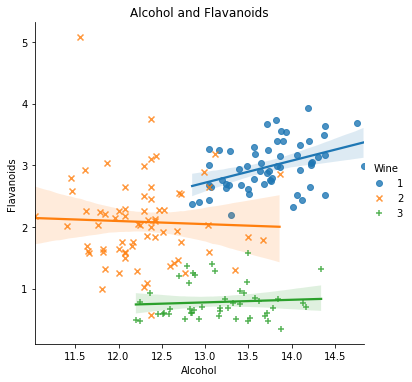
\includegraphics[width = 2in]{Alcohol_Flavanoids.png}
        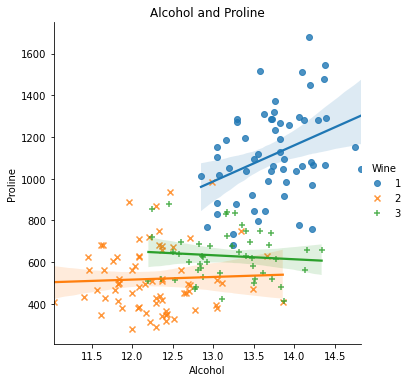
\includegraphics[width = 2in]{Alcohol_Proline.png}
        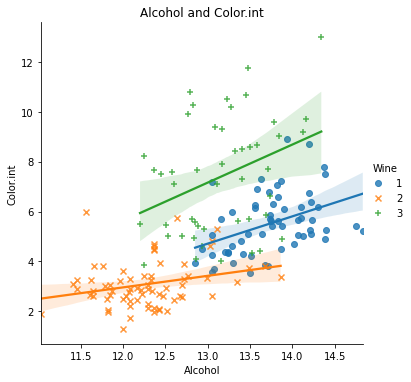
\includegraphics[width = 2in]{Alcohol_Colorint.png} \\
        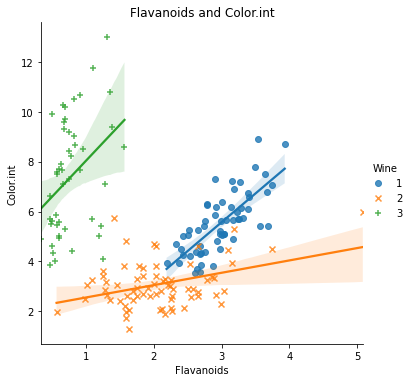
\includegraphics[width = 2in]{Flavanoids_Colorint.png}
        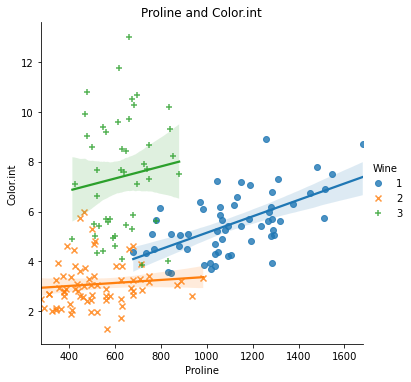
\includegraphics[width = 2in]{Proline_Colorint.png}
        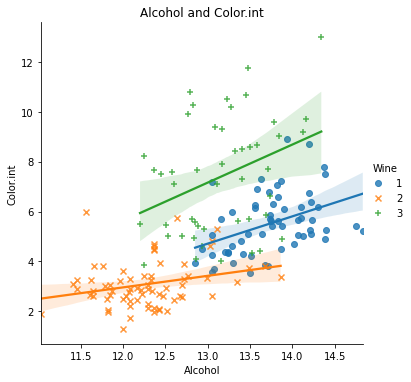
\includegraphics[width = 2in]{Alcohol_Colorint.png}
        \end{center}
    \end{mdframed}
    \item How did you split (i.e., ratio) training vs. testing? 5pt
    \begin{mdframed}
        \begin{itemize}
            \item Training: 80\% (0.8)
            \begin{itemize}
                \item Training size: 142 data points (samples)
            \end{itemize}
            \item Testing: 20\% (0.2)
            \begin{itemize}
                \item Testing size: 36 data points (samples)
            \end{itemize}
        \end{itemize}
    \end{mdframed}
    \item Use ``pickle'' and produce two pkl files. Provide the file names here. 5pt
    \begin{mdframed}
        \begin{itemize}
            \item \verb|wines_train.pkl|
            \item \verb|wines_test.pkl|
        \end{itemize}
    \end{mdframed}
    \item How many $k$'s did you generate? 5pt
    \begin{mdframed}
        I generated $68$ $k$'s.
    \end{mdframed}
    \item How many cross validation scores did you generate? 5pt
    \begin{mdframed}
        I generated $68$ cross validation scores.
    \end{mdframed}
    \item What is the optimal value of $k$ and how did you decide? 5pt
    \begin{mdframed}
        The optimal value of $k$ is $26$ because out of the 68 $k$'s (ranging from 3 to 70) it gave the highest cross validation score of $0.73429$.
    \end{mdframed}
    \item How did your KNN perform? What's your accuracy score? 5pt
    \begin{mdframed}
        My KNN performed mediocrely with an accuracy of $0.72222$.
    \end{mdframed}
\end{enumerate}

% 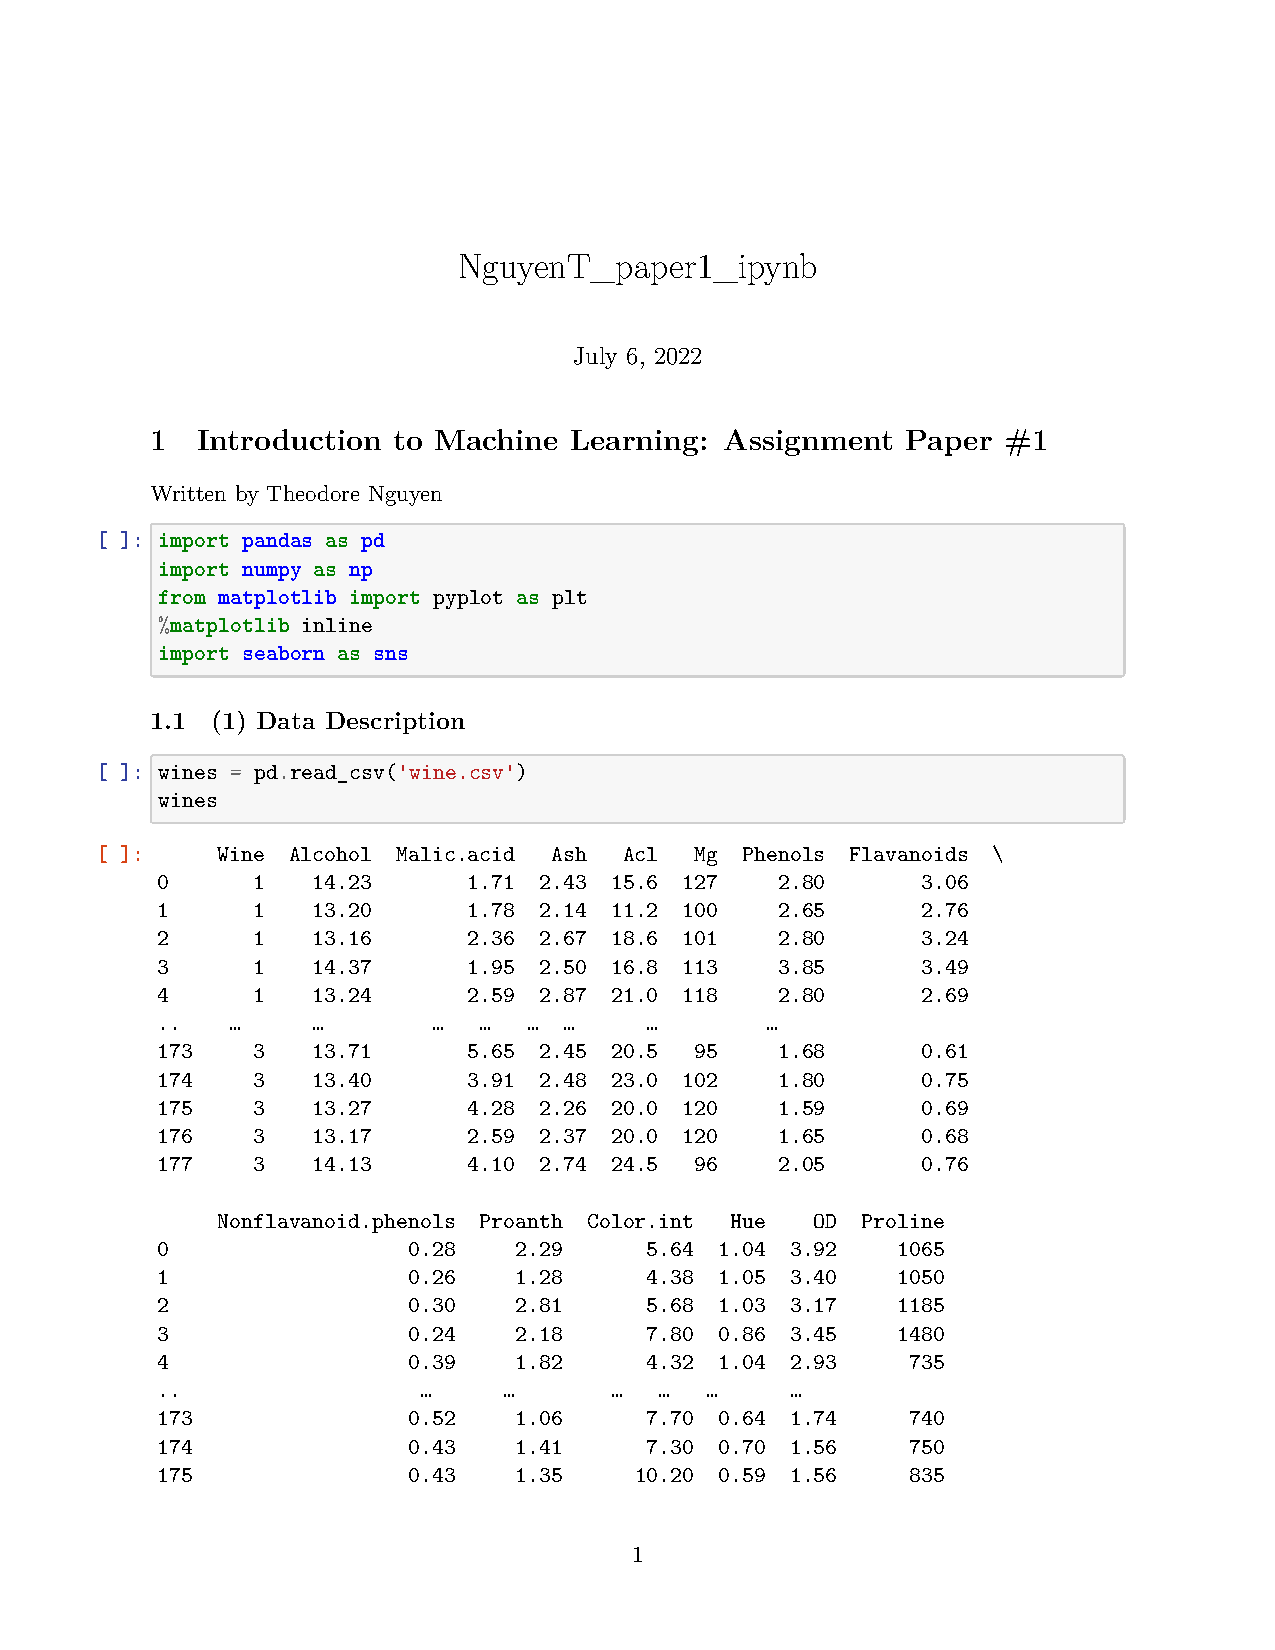
\includepdf[pages = {1-14}]{NguyenT_codes1_ipynb.pdf}

\end{document}